\documentclass[oneside]{htwg-report}

% Use german umlaute
\usepackage{german,ngerman}
\usepackage[T1]{fontenc}
\usepackage[utf8]{inputenc}
\usepackage[ngerman]{babel}
\usepackage[autostyle=true,german=quotes]{csquotes}

%\usepackage[table]{xcolor}\usepackage{float}
%\usepackage{xcolor,colortbl}

\addbibresource{./bib/report.bib}

\begin{document}

\pagenumbering{gobble}

%% 'reporttype' add background elements to the cover / front page
%% possible values are:
%% bachelor	--> B S C
%% master	--> M S C
%% other		--> none
\reporttype{master}

\reporttypetext{Teamprojekt (Master 3. Semester)}

\newcommand{\verfasserA}{Thomas Gnädig}
\newcommand{\verfasserB}{Etienne Gramlich}
\newcommand{\verfasserC}{Merle Wolff}
\newcommand{\verfasserD}{Tim Hardenacke}
\newcommand{\verfasserE}{}
\newcommand{\thema}{DeepRain}
\newcommand{\hoschschule}{Hochschule für Technik, Wirtschaft und Gestaltung}
\newcommand{\institut}{HTWG Konstanz, Institut für Optische Systeme}
\newcommand{\prueferA}{Oliver Dürr}
\newcommand{\prueferB}{}


\title[Teamprojektthema]{\thema}

\doclocation{Konstanz}
\docdate{09. September 2019}

\makecover[]
%          
%% Include an optional title page.
%\begin{titlepage}
\newgeometry{hscale=0.81,vscale=0.8}

\AddToShipoutPicture*{\BackgroundImgTitelPage}

\vspace*{\bigskipamount}


%% Print the title in htwg-teal.
{\makeatletter
\fboxsep=0pt
\colorbox{htwg-white}{\begin{minipage}[t]{145mm}
    \begin{flushleft}
        %% Print Report Type Text
        \color{htwg-teal}\Huge{\@report@typetext}
        \\
        %% Print Report Title
        \color{htwg-teal}\Huge\textbf{\@title}
    \end{flushleft}
\end{minipage}}
\makeatother}

\bigskip
\bigskip

{
\setlength{\parskip}{0.5cm}
\begin{center}
	\textbf{zur Erlangung des akademischen Grades}
	
	\textbf{\Large \type\ of Science (\typeshortcut. Sc.)}
	
	\textbf{an der}
	
	\textsf{\huge Hochschule Konstanz}\\
	{\small Technik, Wirtschaft und Gestaltung}
	
    \textsf{\Large Fakultät Informatik} \\
	Studiengang \studiengang
	
\end{center}
}

\bigskip
\bigskip
\bigskip

\begin{center}
	\begingroup
	\renewcommand*{\arraystretch}{1}
	\rowcolors{2}{white}{white}
	{\makeatletter
		\begin{tabular}{lll}
			\type kandidat: & \verfasser \\
							& \strasse \\
							& \wohnort \\ \\ \\ \\
	
			1. Prüfer: & \prueferA \\
			2. Prüfer: & \prueferB \\ \\ \\ \\
			
			Ausgabedatum: & \ausgabedatum \\
			Abgabedatum: & \abgabedatum
		\end{tabular}
		\makeatother}
	\endgroup
\end{center}


%% reset page margins
\newgeometry{hscale=0.7,vscale=0.8}
\end{titlepage}




\chapter*{Extended Abstract}

\begin{center}
	\begingroup
	\renewcommand*{\arraystretch}{1}
	\rowcolors{2}{white}{white}
	{\makeatletter	
		\begin{tabular}{p{3.2cm}p{9.6cm}}
			Thema: & \thema \\
			& \\
			Teammitglieder: & \verfasserA, \verfasserB \\
			& \\
			Betreuer: & \hoschschule \newline \institut \newline \prueferA, \prueferB \\
			& \\
		\end{tabular}
		
		\makeatother}
	\endgroup
\end{center}

\bigskip

We try to predict precipitation for a range of 35 minutes in an area around Constance.
Therefore we are using machine learning techniques and train a UNet on radar data images. 
Here we present the result of precipitation prediction as well with regression as with classification. 
Both approaches provide good results.


\printbibliography[title={Referenzen}, heading=subbibliography]


\twocolumn
\section*{Data}
We are using radar Data from the Climate Data Center of the DWD\footnote{\url{https://www.dwd.de/DE/klimaumwelt/cdc/cdc_node.html}}. Here are radarimages since 2004. 
This data has to be Downloaded and converted to png this is done by our Crawler\footnote{\url{https://github.com/thgnaedi/DeepRain/tree/master/DWD_Crawler}} and Converter\footnote{\url{https://github.com/thgnaedi/DeepRain/blob/master/Data/DWDtoPngScript.py}}.
The rainfall images then are tailored and scaled. Unattraktive images are then rejected that only interessting images are used for the training.
The images are grayscale png's. As network input five temporally consecutive of them are combined to a 3D tensor as input. The label consists of seven of them.

\section*{Architecture}
To predict precipitation either with regression or classification we are using a UNet.
This Architecture is a convolutional neural network that was at first developed for biomedical image segmentation.
A UNet is a set of convulution layers, combined with an downsampling part, such as pooling layers, and later with upsampling parts like deconvolution layers.

\begin{figure}[ht]
\centering
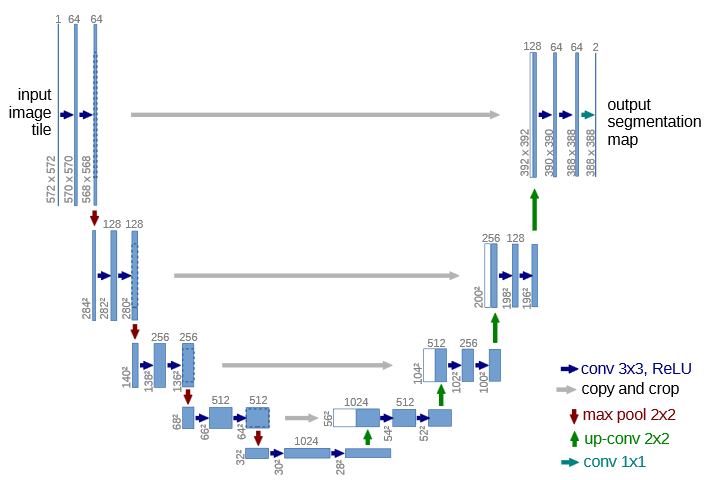
\includegraphics[width=0.8\linewidth]{../pics/UNet_Biomedical}
\caption{The image is taken from the university of Freiburg~\cite{ronneberger2015u}}
\end{figure}

The input images have a shape of 64x64 pixels. They are pooled until the shape reaches a minimum of 8x8 features. Then they are upsampled and concatenated with the downsampling part.
This yields into an u-shaped architecture with crosslinks and is the reason for its name.

\section*{Regression}
First approache is to predict the complete radar image. For this regression we use the MSE as lossfunction. The input layer takes the five incoming timesteps and transfers it into a 7 timestep prediction wich reaches up to 35 minutes into the future.
Our network is trained on the radar data from 2005 till 2017. As validation set we use the images from 2004. further information can be found in our full project description\footnote{\url{https://github.com/thgnaedi/DeepRain/blob/master/Docs/Langdokumentation.pdf}}.
The result of this task is shown in the following graphics.

\begin{figure}[ht]
\centering
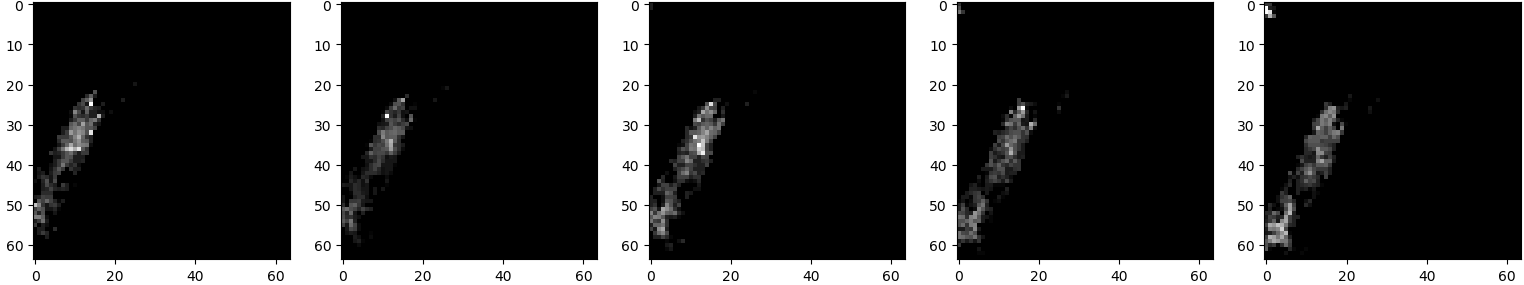
\includegraphics[width=\linewidth]{../pics/dt5}
\caption{The input is a 64x64x5 Tensor, containing the last 25 minutes, with the following content}
\end{figure}


\begin{figure}[ht]
\centering
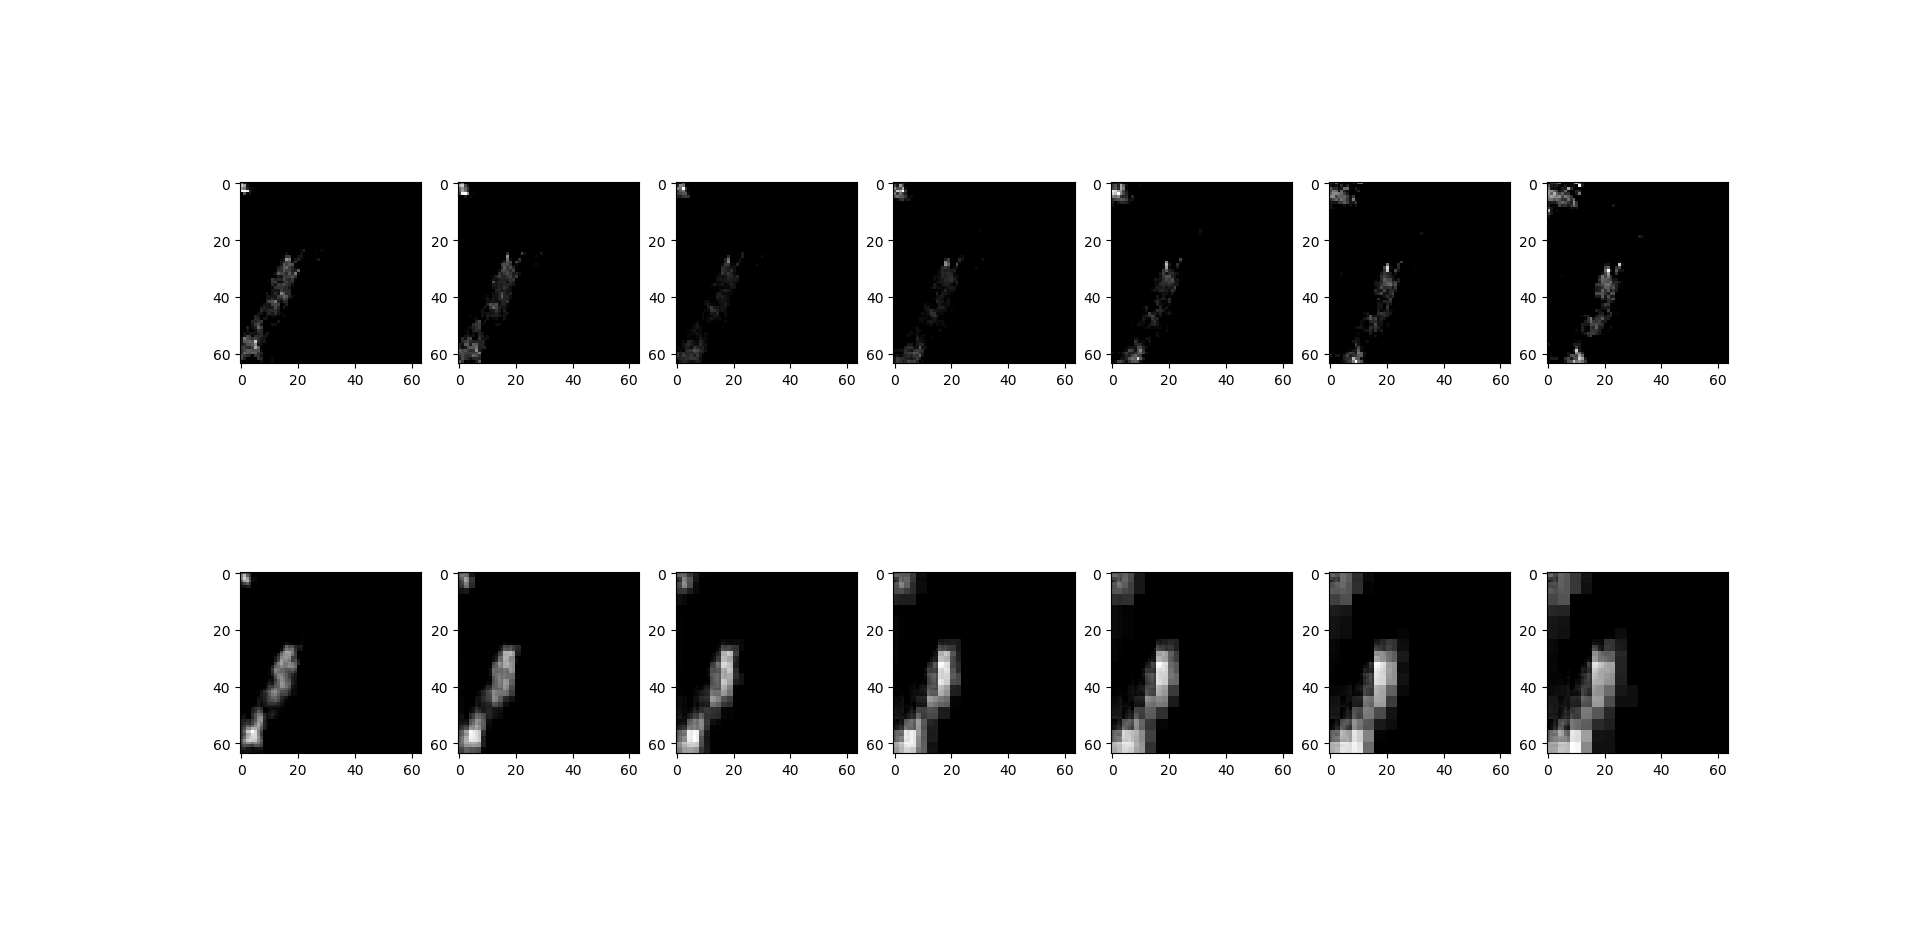
\includegraphics[width=\linewidth]{../pics/t5}
\caption{The Labels are seven timesteps to predict, from 5 minutes till 35 minutes into the future. The result is shown here. In the upper row we can see the seven timesteps in the Labels. White means a lot rainfall while black is no rainfall.
The second row contains the labels for this input. In the last row are the predictions of our model.}
\end{figure}

The predicted values are very close to the label for a difference of only 5 minutes to the input data. The further the time progresses, the worse the prediction becomes.
In the last image it looks like the resolution of the output has been drastically decreased compared to the first output. 
In fact the resolution is the same we can say that this is an indication of uncertainty in the Network.
Over the time, the movement of the rainfall is well predicted. even the tiny spot in the top left of Images can be predicted.
Even if the area of rainfall increases much faster than in the labels, the center is still well predicted and close to the center of the label.

\section*{Classification}
The second approach is to predict the precipitation by classification. Here we try to classify into either three classes (no rain, rain, heavy rain) or two classes (no rain, rain) for each pixel.
Herefore the Unets output is modified to three classes per pixel and an additional softmax layer at the output to provide propabilities. The labels are generated by a threshold for each class.

\begin{figure}[ht]
\centering
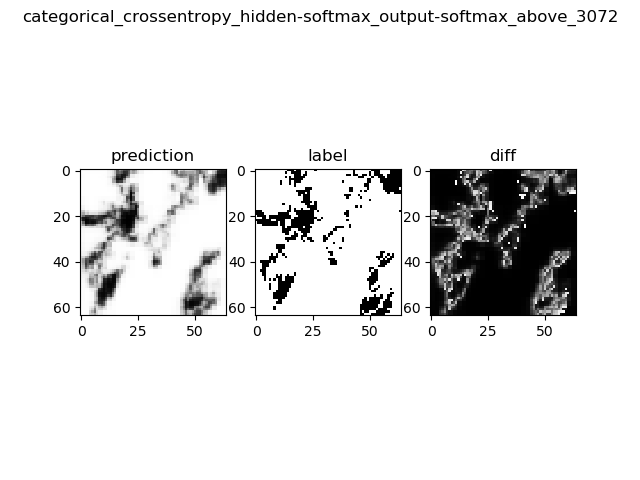
\includegraphics[width=\linewidth]{../pics/categorical_crossentropy_hidden-softmax_output-softmax_above_3072}
\caption{classification output. in the left image the prediction of the first class (no rainfall) is plotted. The white spots are 100\% no rainfall. the black spots are 0\% no rainfall.}
\end{figure}


The gray spots can be rainfall or not depending on the propability of the other two classes. The right image (difference) shows us the absolute difference between the prediction and the label.
Here we can see that the big black spots (no difference between prediction and label) are at the no rainfall labels. This can be explained later. 
The network has a high accuracy by predicting rainfree pixels. this can be shown in the follwing ROC-image. 
By evaluating the confusion matrix for three class classification, you can recognize that the last class (heavy rainfall) is higly undersampled. 
There are much more rainfall pixels and even more no rainfall pixels in the Dataset. To increase the the performance we tried over and undersampling, but both tecniques didnt work well for our scenario.
Finally we changed the problem to a two clas classification with a threshold of 0, so the classes are 'no rainfall' and 'rainfall'.


\begin{figure}[ht]
\centering
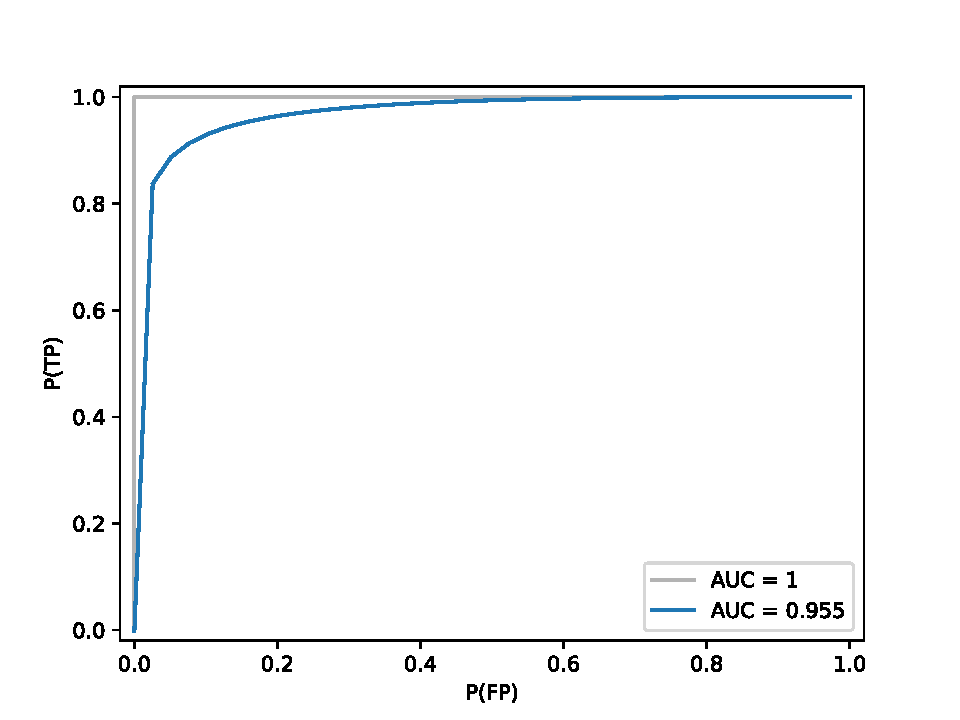
\includegraphics[width=\linewidth]{../pics/ROC-curve}
\caption{To show the performance you can take a lock at the ROC. The calculated AUC is close to 96\%, wich means, that the model has a good class separation.}
\end{figure}

\section*{Conclusion and Future Work}
In summary, this paper argued that short term precipitation prediction can be done by only observing radar data and without any other source of information.
The accuracy could still be imporved as well at the regression, were another lossfunction may could help, as at the classification were the rainfall class is still undersampled and worse accurate than the 'no rain' class.

\end{document}

